% =====================================================================
% FLAIR --- NEJM AI Datasets, Benchmarks, and Protocols
% Version 3 (rewrite). Self-contained manuscript source.
%
% Structure: IMRAD for a Datasets/Benchmarks/Protocols article.
% Main-text display items (NEJM AI cap = 5): Figure 1 (workflow),
% Table 1 (task suite), Table 2 (consortium cohort), Figure 2 (forest),
% Figure 3 (degradation). All other tables/figures are in the appendix.
%
% ILLUSTRATIVE DATA: MIMIC-CLIF and Rush are observed FLAIR v2 results.
% Sites C--H are illustrative projections (flagged with a dagger and named
% as such in every caption); they are not collected data. All numbers are
% single-sourced from flair_paper_data.py.
% =====================================================================

\documentclass[12pt]{article}

\usepackage[margin=1in]{geometry}
\usepackage[T1]{fontenc}
\usepackage{lmodern}
\usepackage{microtype}
\usepackage{setspace}
\usepackage{booktabs}
\usepackage{tabularx}
\usepackage{graphicx}
\usepackage{enumitem}
\usepackage{xcolor}
\usepackage[hidelinks]{hyperref}
\usepackage[round]{natbib}

\doublespacing
\setlength{\parskip}{0.3em}
\setlength{\parindent}{0pt}

% Placeholder marker for the handful of items that need author sign-off
% before submission. Rendered distinctly so it cannot be mistaken for prose.
\newcommand{\confirm}[1]{\textcolor{gray}{[\textsc{author}: #1]}}

\title{\textbf{FLAIR: A Federated ICU Benchmark for External Validation on the Common Longitudinal ICU Format}}
\author{CLIF Consortium \\ FLAIR Working Group}
\date{\today}

\begin{document}
\maketitle

\begin{abstract}
\noindent\textbf{Background.} Clinical decision-support models for the intensive care unit (ICU) are produced far faster than the multi-site evidence needed to judge whether they work in hospitals that did not build them. Public ICU benchmarks accelerate development but centralize their test data, so they inherit one source's biases and can saturate under repeated tuning. Traditional external validation requires bilateral data-use agreements and patient-level data transfer, and rarely scales beyond a few sites.

\noindent\textbf{Methods.} FLAIR is an open-source federated benchmark and model-to-data protocol for ICU prediction. It is built on the Common Longitudinal ICU Format (CLIF), a critical-care data standard with shared tables and mCIDE categories. Developers build against public MIMIC-CLIF; after Benchmark Committee review, byte-identical code runs locally at participating CLIF sites, and only aggregate, cell-suppressed report bundles return. Five binary tasks are included: daily in-hospital mortality, daily long-term acute-care hospital (LTACH) discharge, extubation failure within 24 hours, CDC Adult Sepsis Event within 6 hours, and unplanned ICU readmission. A single frozen XGBoost count-feature model serves as the reference baseline.

\noindent\textbf{Results.} The baseline trained on MIMIC-CLIF reached internal AUROCs of 0.864, 0.789, 0.696, 0.693, and 0.641 across the five tasks, but degraded on every task at the first external site (Rush): 0.748, 0.658, 0.565, 0.407, and 0.509. Sepsis discrimination fell below chance externally. An illustrative eight-site consortium projects the same failure mode as a distribution, not an anecdote, with the largest internal-to-external gap for sepsis.

\noindent\textbf{Conclusions.} FLAIR makes multi-site ICU evaluation reproducible, auditable, and feasible without routine patient-level data transfer. It is a benchmark and protocol resource, not evidence of clinical utility for any specific model.
\end{abstract}

\section{Introduction}

The bottleneck in ICU clinical AI is no longer the supply of models; it is trustworthy evidence that a model works somewhere it was not built. Predictive algorithms for sepsis, acute kidney injury, extubation readiness, mortality, and hospital operations appear continually, but whether a given model behaves acceptably outside its development hospital is often unknown. That evidence gap is, in large part, an access gap: representative multi-institutional ICU data are rarely available to the team that needs to test a model.

External validation of flagship electronic health record (EHR)-based decision support has stayed narrow and slow. The Epic Sepsis Model, deployed across many United States hospitals, was first independently evaluated at a single site, where discrimination fell to an AUC of 0.63 against vendor-claimed ranges of 0.76 to 0.83 \citep{wong2021external,habib2021jamaeditorial}. Duke's Sepsis Watch and the Targeted Real-time Early Warning System each required years and reached only a handful of sites \citep{sendak2025sepsiswatchportability,adams2022trews}; Mayo Clinic's electrocardiogram screen needed multi-year coordination to cover several external sites \citep{carter2025mayoecgai}. Serious validation is possible, but it does not keep pace with model production.

Public benchmarks help but cannot close the gap alone. ICU benchmarks built on MIMIC, eICU, HiRID, and AUMCdb are essential for reproducible development \citep{vandewater2023yaib,yeche2021hirid,pollard2018eicu}, yet they centralize their test data, inherit its selection biases \citep{roosli2022mimicfairness}, and can make performance look more transportable than it is once the same public set is tuned against repeatedly \citep{recht2019imagenet,chekroud2024illusory}. This is precisely the ``why not just use an existing benchmark'' question: EHRSHOT and the FEMR tokenization tradition offer a public few-shot benchmark that FLAIR builds on for its baseline representation \citep{wornow2023ehrshot,steinberg2021femr}, and the Medical Event Data Standard offers a data standard \citep{arnrich2025meds}, but none provides a standing, ICU-scoped, \emph{federated validation} layer over data that never leaves the hospital.

Several communities show pieces of a better approach. OHDSI and LEGEND federate studies across OMOP \citep{reps2020ohdsistroke}; MedPerf orchestrates model-to-data imaging benchmarks \citep{karargyris2023medperf}; the FeTS Challenge federated imaging \emph{training} \citep{pati2022fets}; OpenSAFELY moves analytic code to national primary-care data without moving rows \citep{opensafely2021naturemedicine}; and DREAM and EHR DREAM turned model-to-data evaluation into a challenge format \citep{guinney2018dream,bergquist2024ehrdream}. What has been missing for ICU EHR decision support is the combination of a critical-care data standard, a reusable task catalog, and a standing federated protocol.

FLAIR (Federated Learning Assessment for ICU Research) supplies that combination. The idea is simple: the model goes to the data, and aggregate evaluation reports come back. A developer writes code against MIMIC-CLIF, the public CLIF expression of MIMIC-IV \citep{johnson2023mimiciv,johnson2016mimiciii}; after review, the same code runs inside each site, which returns tables and metrics, not patient rows. We describe FLAIR as three coupled artifacts---a data layer (CLIF, with MIMIC-CLIF as the public entry point), a task layer (five inspectable Python tasks with an open catalog), and a protocol layer (committee-reviewed, aggregate-only model-to-data execution)---and we show that even a simple reference baseline already exposes large, task-dependent cross-site degradation. FLAIR does not certify models for bedside use; its purpose is to make multi-site ICU evaluation reproducible, auditable, and feasible without routine patient-level data transfer.

\section{Methods}
\label{sec:methods}

\subsection*{Data layer: CLIF and MIMIC-CLIF}

CLIF harmonizes ICU EHR content into a limited set of relational tables with mCIDE category definitions \citep{rojas2025clif}, covering patients, hospitalizations, admission-discharge-transfer (ADT) events, vitals, labs, medications, respiratory support, patient assessments, microbiology, and diagnoses. Because task code refers to shared table names and category values, it reduces the site-specific feature engineering otherwise required before a model can be evaluated. In spirit CLIF is to critical care what mCODE is to oncology---a clinically scoped common-data-element layer that makes analytic code portable \citep{mcode2024hl7}---and it is complementary to broader EHR event standards such as the Medical Event Data Standard \citep{arnrich2025meds}. MIMIC-CLIF, the public development dataset, expresses MIMIC-IV in the CLIF v2.1 schema and contains approximately 72{,}800 ICU stays \citep{johnson2023mimiciv}. Developers use it to debug task definitions, train baselines, and confirm that submissions follow the cohort and prediction-file contracts before any federated execution, yielding a develop-on-public, validate-on-private workflow.

\subsection*{Task layer: five ICU tasks}

Each task is a single Python module with a \texttt{META} dictionary (task class, temporal pattern, prediction unit, label, clinical threshold, direction, report mode) and a \texttt{build()} function returning one row per prediction opportunity. Every row carries a stable \texttt{prediction\_id}, a stitched-encounter key, a prediction timestamp (\texttt{prediction\_dttm}, the no-future-data boundary), the label, the train/test split, and demographics for reporting. The five tasks (Table~\ref{tab:taskspec}) span outcome, disposition, respiratory, infectious-deterioration, and utilization questions \citep{thille2011extubation,rojas2018readmission}. Task~4 predicts onset of a CDC Adult Sepsis Event \citep{rhee2019sepsis} within 6 hours on an hourly hospital-wide grid, using the CLIF Adult Sepsis Event utility with lactate and the \texttt{microbiology\_culture} table, and stopping strictly before onset; it follows the before-treatment sepsis formulation of \citet{kamran2024sepsis} and contrasts with antibiotic-anchored Sepsis-3 definitions \citep{singer2016sepsis3,seymour2016assessment}. The catalog is designed to grow: any contributor can propose a task as a module, and acceptance requires MIMIC-CLIF reproducibility, clinician-led face-validity review, and site-governance sign-off at a minimum of two sites---a structural counter to benchmark saturation.

Three methodological safeguards make cohorts comparable across sites. First, fragmented encounters (e.g., emergency-department to inpatient transfer, or discharge and rapid readmission) are stitched into a single unit, \texttt{hospitalization\_join\_id}, using a 6-hour gap rule, so one clinical episode is never split across the train/test boundary. Second, features may use only data at or before \texttt{prediction\_dttm}. Third, splits are assigned at the stitched-encounter grain (75/25): MIMIC-CLIF uses a deterministic hash split because its admission dates are de-identified, while other sites use a temporal split (oldest 75\% train, newest 25\% test). A SHA-256 audit hash over the task source and its policy metadata is stamped into every report, so sites can prove they ran identical task code.

\begin{table}[t]
\centering
\footnotesize
\setlength{\tabcolsep}{5pt}
\begin{tabular}{llllll}
\toprule
\textbf{Task} & \textbf{Outcome} & \textbf{Prediction grid} & \textbf{Report mode} & \textbf{Threshold} & \textbf{Prev.} \\
\midrule
T1 & ICU daily mortality       & daily 07:00      & landmark & 0.95 (above) & 0.134 \\
T2 & LTACH discharge           & daily 07:00      & landmark & 0.50 (above) & 0.065 \\
T3 & Extubation failure 24 h   & at extubation    & episodic & 0.15 (below) & 0.054 \\
T4 & Sepsis (CDC ASE) 6 h      & hourly           & peak     & 0.10 (above) & 0.063 \\
T5 & Unplanned ICU readmission & at ICU discharge & episodic & 0.20 (above) & 0.093 \\
\bottomrule
\end{tabular}
\caption{The five FLAIR benchmark tasks. Prevalence is the stay-level positive rate on MIMIC-CLIF. Clinical thresholds and directions are single-sourced in the package policy registry and folded into each task's audit metadata. Report modes are defined in the text. Source: FLAIR task code and v2 baseline artifacts.}
\label{tab:taskspec}
\end{table}

\subsection*{Reference baseline}

The reference baseline is one frozen XGBoost model over point-in-time count features, in the EHRSHOT/FEMR tradition \citep{wornow2023ehrshot,steinberg2021femr}. CLIF events are converted to a fixed 211-code Event List Format vocabulary; each prediction row is represented by counts of codes observed strictly before \texttt{prediction\_dttm}, with numeric and categorical codes truncated so that units are never features and discharge diagnoses excluded to prevent leakage. Hyperparameters are tuned once on MIMIC-CLIF (Optuna, 30 trials, 5-fold cross-validated AUROC; see Appendix). The trained model and token dictionary are then shipped unchanged to each site for inference only; there is no per-site training. These values are benchmark checks, not a claim that the baseline is clinically adequate.

\subsection*{Evaluation modes}

Because continuous ICU tasks can be scored in more than one clinically meaningful way, FLAIR separates task construction from scoring mode. \emph{Episodic} scoring is used when there is one prediction per stay (T3, T5). \emph{Landmark} scoring is used for daily trajectories (T1, T2) and reports performance at lead-time slices before the stay endpoint. \emph{Peak} scoring is used for continuous screening (T4): it collapses each stay to its highest predicted risk before computing discrimination and subgroup metrics. Calibration and decision-curve analysis are omitted under peak scoring because taking the maximum of many probabilities distorts calibration. This distinction is load-bearing---a row-level metric can overstate the performance a unit would experience acting on one alarm per stay. All metrics are scored on the held-out test split with percentile-bootstrap 95\% confidence intervals resampled at the stay level.

\subsection*{Protocol layer: federated execution and governance}

The protocol makes FLAIR's privacy properties operational (Figure~\ref{fig:workflow}). A \textbf{Model Owner} submits a frozen model, code folder, or container developed against MIMIC-CLIF. The \textbf{Benchmark Committee}---clinicians, methodologists, and site data stewards---reviews submissions for reproducibility, clinical face validity, and security, and stamps an audit hash before dispatch. The \textbf{FLAIR Portal} registers tasks, models, and versions, distributes byte-identical artifacts, collects reports, and renders the leaderboard. At each institution, a \textbf{Site Lead or Data Steward} runs the approved artifact locally against site CLIF tables and returns only the standardized non-PHI report bundle. Three properties define the access model: no patient-level data leave any site; the library enforces suppression (cohort counts below 10 suppressed, subgroups with fewer than 10 observations omitted, sparse calibration bins withheld); and governance review precedes execution, with sites retaining final approval over what runs locally. Each report bundle carries cohort summaries, discrimination, calibration and decision curves where applicable, subgroup and lead-time summaries, a suppressed code registry, and audit metadata (task name, task hash, package version, report mode, split, number of stays, prevalence, and operating threshold). This model-to-data pattern follows the DREAM and EHR DREAM lineage \citep{guinney2018dream,bergquist2024ehrdream}; FLAIR's contribution is to make it a standing ICU benchmark. Reporting follows the structure expected of clinical prediction models \citep{collins2024tripodai}, with a Datasheet framework for the public cohort \citep{gebru2021datasheets} and a Model Card framework for the baseline \citep{mitchell2019modelcards}.

\begin{figure}[t]
\centering
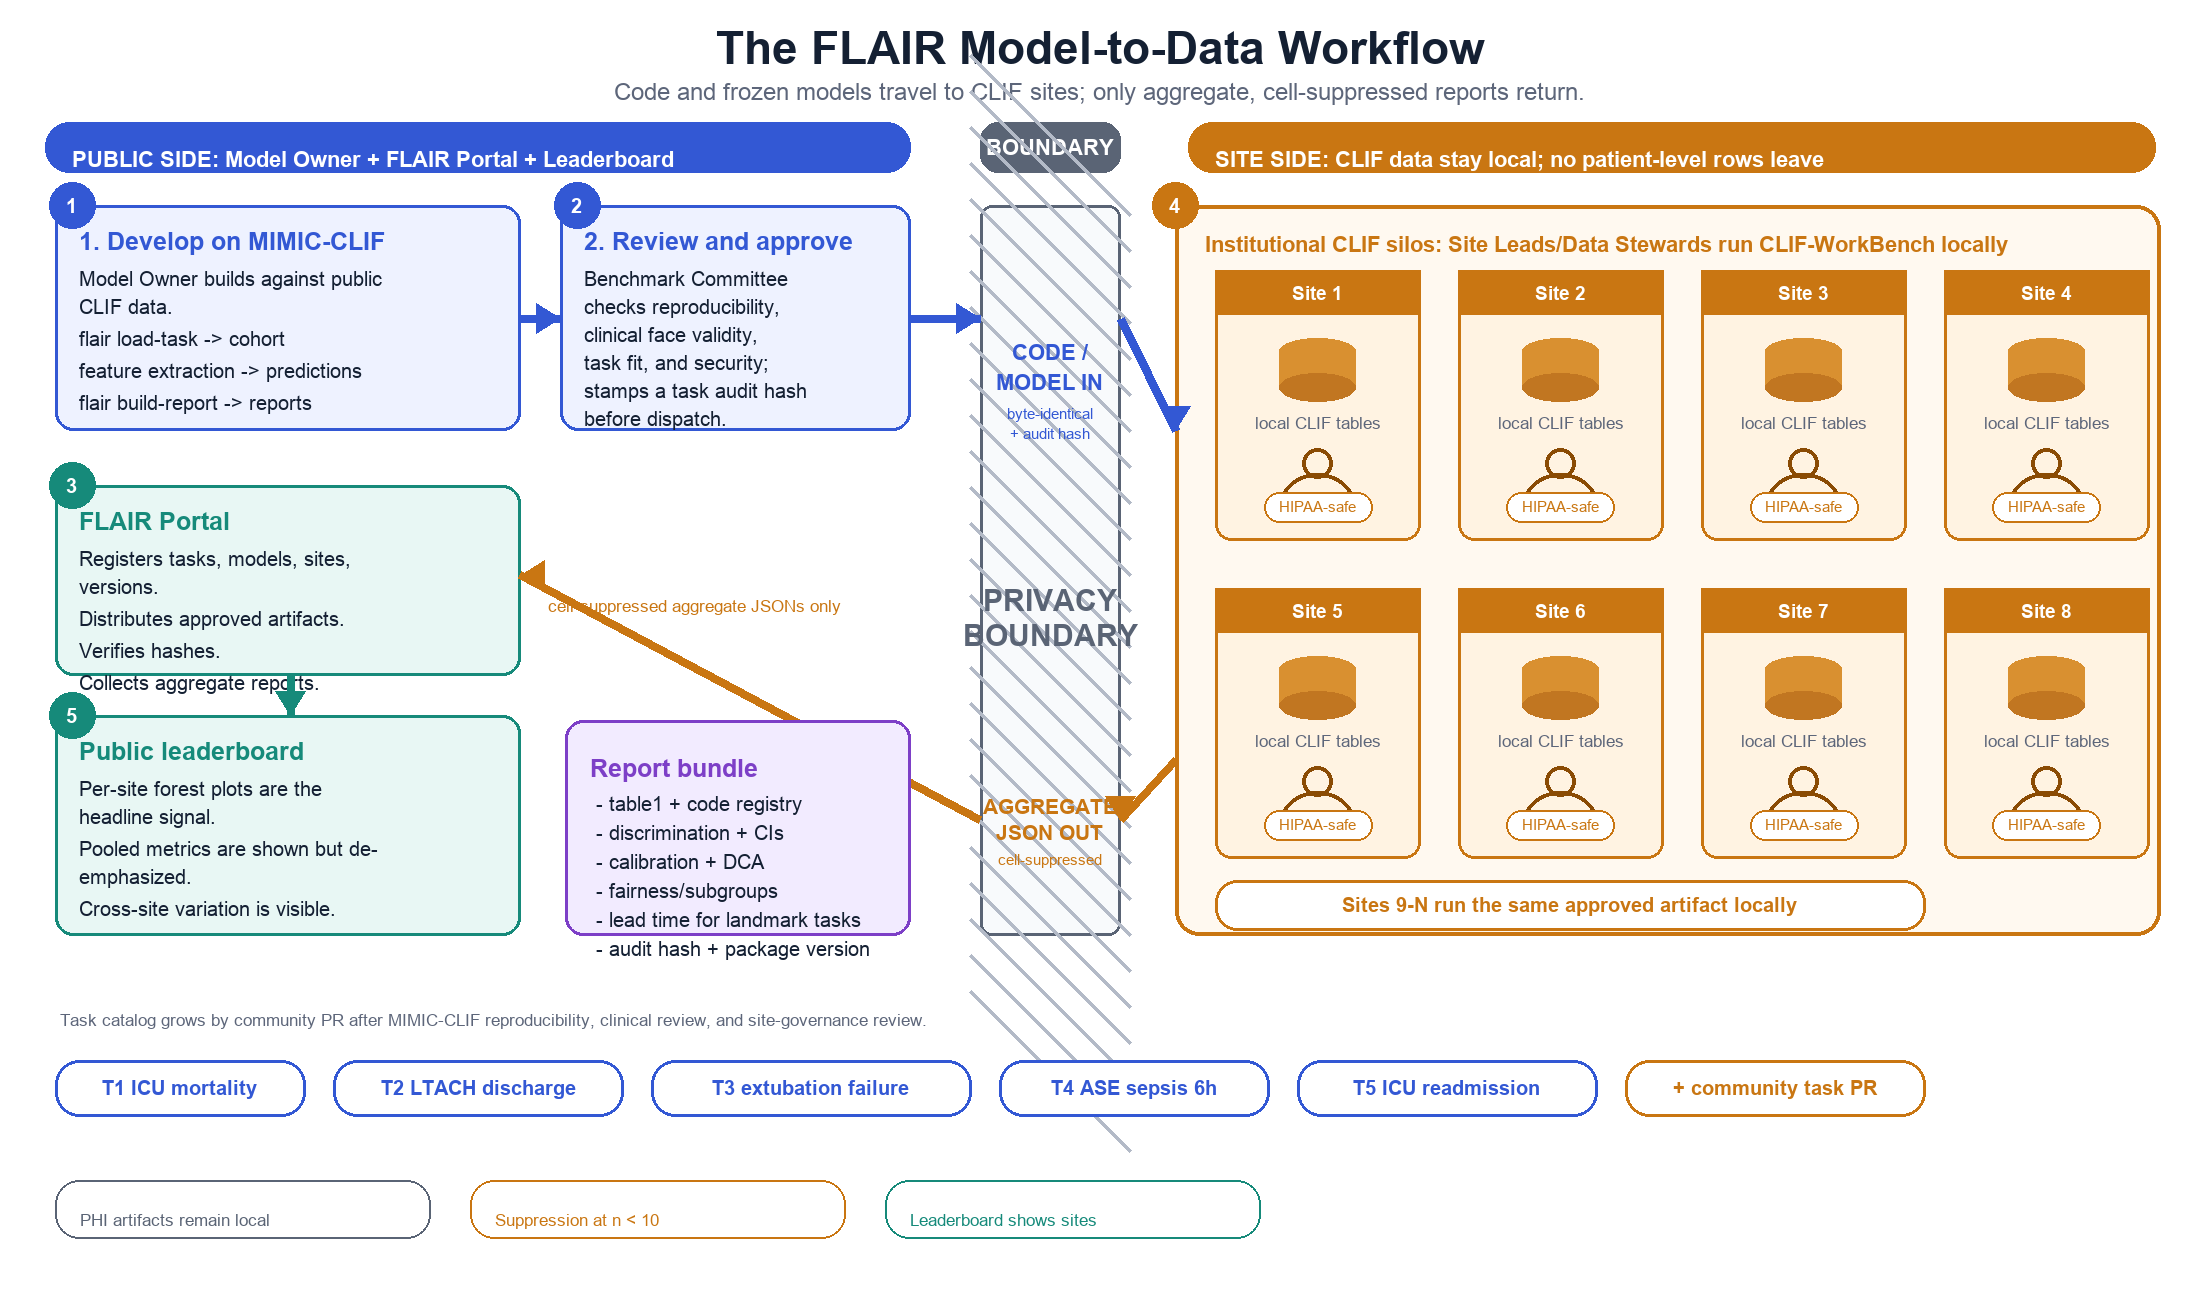
\includegraphics[width=\linewidth]{figures/figure1_flair_workflow_v3.png}
\caption{The FLAIR model-to-data loop. A Model Owner develops against public MIMIC-CLIF and submits a frozen model, code, or container. The Benchmark Committee reviews it for reproducibility, clinical face validity, and security, and stamps a task audit hash. The FLAIR Portal distributes byte-identical code to participating CLIF sites, where a Site Lead or Data Steward runs it locally against site CLIF tables. Patient-level cohorts, features, and predictions remain inside the institutional boundary; only aggregate, cell-suppressed JSON report bundles return. The leaderboard foregrounds per-site variation rather than a single pooled scalar. Source: authors.}
\label{fig:workflow}
\end{figure}

\section{Results}
\label{sec:results}

\subsection*{Consortium cohort}

Table~\ref{tab:consortium} describes the cohort. MIMIC-CLIF and Rush report observed results; the remaining six sites (C--H) are illustrative academic-medical-center archetypes shown to convey the intended consortium and are not collected data. Together the eight sites represent approximately 187{,}600 ICU stays across a range of case mixes---quaternary academic, community-academic, urban safety-net, and rural referral---with median age from 58 to 69 years and female proportion from 43\% to 48\%. This heterogeneity is the setting in which transportability, rather than internal accuracy, is the relevant question.

\begin{table}[t]
\centering
\footnotesize
\setlength{\tabcolsep}{5pt}
\begin{tabular}{llrrrr}
\toprule
\textbf{Site} & \textbf{Archetype} & \textbf{ICU stays} & \textbf{Female \%} & \textbf{Age} & \textbf{SOFA} \\
\midrule
MIMIC-CLIF & Public development (MIMIC-IV) & 72{,}778 & 43.2 & 67 & 5 \\
Rush       & Urban academic medical center & 13{,}839 & 47.5 & 65 & 4 \\
Site C$^\dagger$ & Northeast quaternary academic & 24{,}610 & 44.1 & 63 & 6 \\
Site D$^\dagger$ & Midwest urban safety-net      & 11{,}205 & 46.3 & 58 & 5 \\
Site E$^\dagger$ & Southern community-academic   & 18{,}470 & 48.2 & 64 & 5 \\
Site F$^\dagger$ & West Coast academic           & 22{,}400 & 44.9 & 63 & 5 \\
Site G$^\dagger$ & Rural referral center         &  8{,}720 & 45.0 & 69 & 4 \\
Site H$^\dagger$ & Mixed academic-community      & 15{,}600 & 47.1 & 65 & 5 \\
\bottomrule
\end{tabular}
\caption{Federated consortium cohort characteristics. Age is the median in years; SOFA is the median hospital-maximum score. \textbf{MIMIC-CLIF and Rush are observed} FLAIR v2 results; \textbf{sites marked $^\dagger$ (C--H) are illustrative projections pending federated runs and are not collected data.} Per-site cell suppression at $n<10$ is applied. Source: FLAIR v2 baseline artifacts (observed) and \texttt{flair\_paper\_data.py} (illustrative).}
\label{tab:consortium}
\end{table}

\subsection*{Cross-site degradation}

The central finding is observed and unambiguous: the frozen baseline degraded on all five tasks from the MIMIC-CLIF internal holdout to the first external site (Figure~\ref{fig:degradation}). AUROC fell by 0.116 for daily mortality (0.864 to 0.748), 0.131 for LTACH discharge (0.789 to 0.658), 0.131 for extubation failure (0.696 to 0.565), 0.132 for readmission (0.641 to 0.509), and 0.286 for sepsis (0.693 to 0.407). Sepsis discrimination fell below chance at the external site---the number a developer sees internally is not the number a new hospital gets. Because Task~4 is a rare, hospital-wide, hourly screening task, it is both the most clinically consequential and the most fragile under distribution shift.

Figure~\ref{fig:forest} places these observed anchors in the context of the projected consortium. Across the external sites, the illustrative median AUROC is below the MIMIC-CLIF internal value for every task, and the internal-to-external gap is largest for sepsis (median 0.559; gap 0.134) and smallest for daily mortality (median 0.789; gap 0.075). Two external sites fall below chance on sepsis. The point of the display is not any single site's number but the spread: a single pooled AUROC would hide the failure mode FLAIR exists to surface, whereas a per-site forest plot makes it the headline. Full per-site metrics, calibration, decision curves, lead-time, and subgroup results are provided in the Appendix.

\begin{figure}[t]
\centering
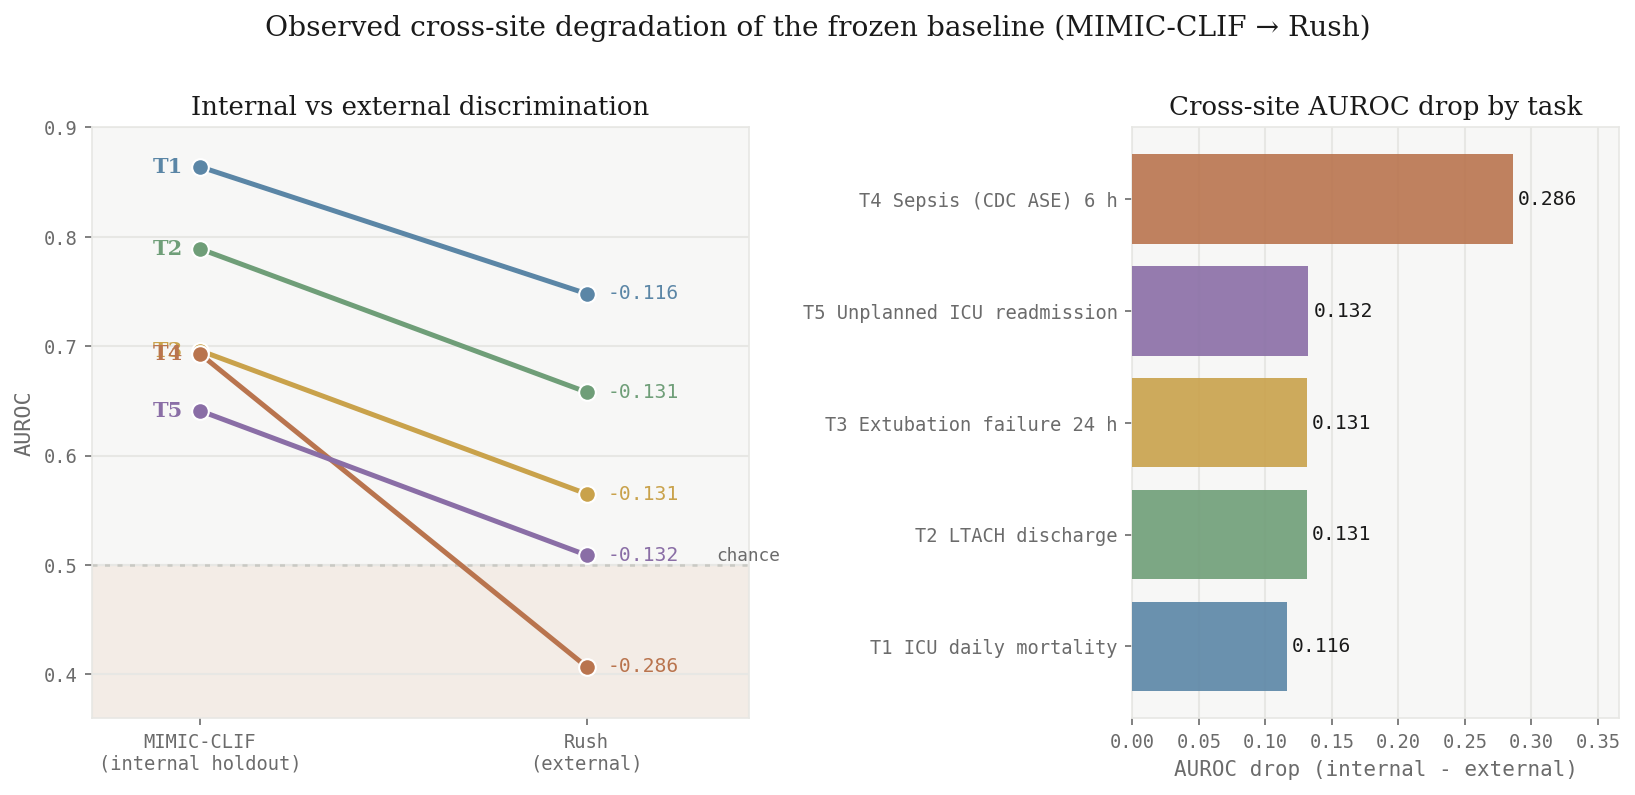
\includegraphics[width=0.92\linewidth]{figures/figure3_degradation.png}
\caption{Observed cross-site degradation of the frozen baseline from the MIMIC-CLIF internal holdout to the first external site (Rush). Left: AUROC for each task falls from internal to external; sepsis crosses below the chance line. Right: the internal-to-external AUROC drop by task, ordered by magnitude. Both panels use only observed data. Source: FLAIR v2 baseline artifacts.}
\label{fig:degradation}
\end{figure}

\begin{figure}[t]
\centering
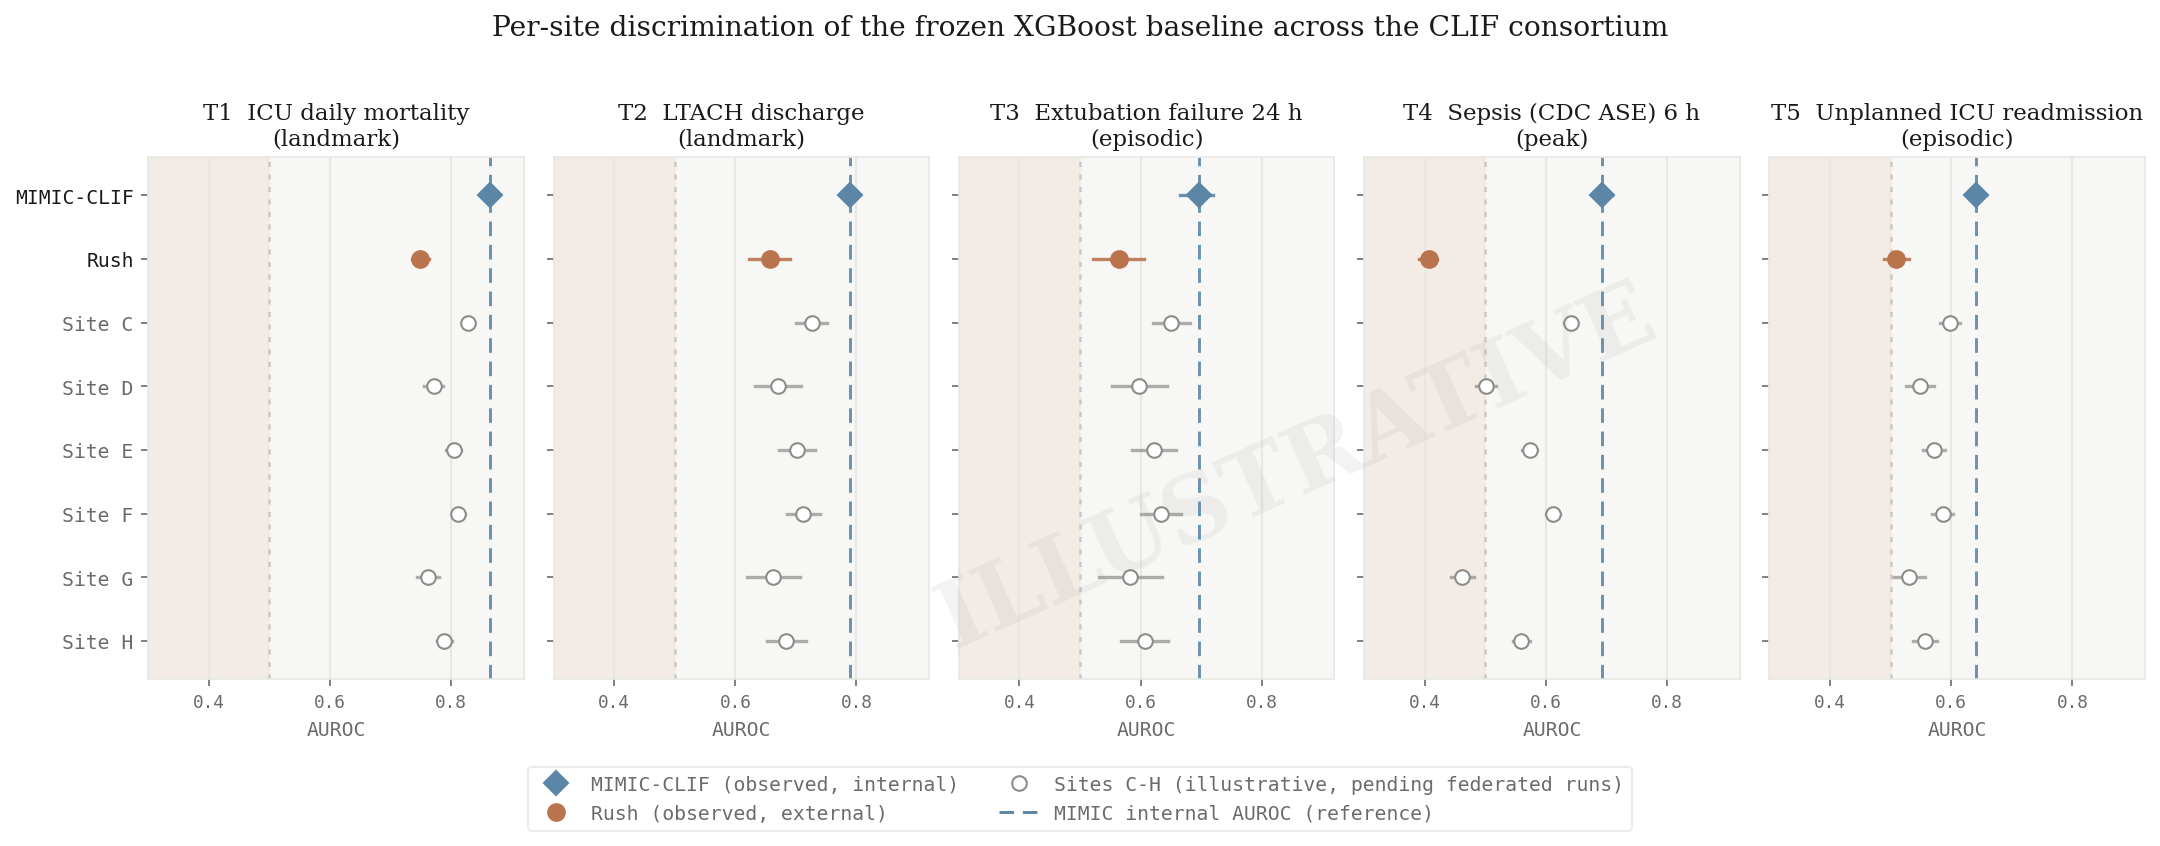
\includegraphics[width=\linewidth]{figures/figure2_forest_auroc.png}
\caption{Per-site discrimination of the frozen baseline across the CLIF consortium, one panel per task. Each marker is a site's AUROC with a 95\% confidence interval; the dashed line is the MIMIC-CLIF internal reference and the shaded band marks worse-than-chance discrimination. \textbf{MIMIC-CLIF (blue) and Rush (terracotta) are observed}; \textbf{open grey markers (Sites C--H) are illustrative projections pending federated runs}, as noted by the watermark. Source: FLAIR v2 baseline artifacts (observed) and \texttt{flair\_paper\_data.py} (illustrative).}
\label{fig:forest}
\end{figure}

\section{Discussion}

FLAIR combines three properties that have appeared separately but not together at the scale ICU clinical AI requires: evaluation across heterogeneous hospitals without patient-data movement, a clinically scoped ICU data standard that makes code portable, and a governance protocol that lets the task catalog grow through community contribution. The empirical payoff is already visible in a deliberately simple baseline: strong internal discrimination does not survive the trip to a hospital that did not build the model, and the degradation is task-dependent, with sepsis screening the most fragile. This is consistent with a large literature on dataset shift in clinical prediction \citep{finlayson2021clinicianshift}, but FLAIR turns that observation from a warning into a measurement.

\paragraph{Saturation resistance and the regulatory posture.} Because FLAIR's test data remain siloed at participating sites, the data underlying the leaderboard never enter public hands, which limits the risk that future models are pretrained on the evaluation set and reduces the incentive to tune to a private test set that cannot be seen \citep{recht2019imagenet,chekroud2024illusory}. FLAIR also federates \emph{evaluation} rather than \emph{training}: aggregate, cell-suppressed metrics leak less patient information than the model updates exchanged in federated learning, and there is no per-site trained model object to share. This positions FLAIR as a structural contribution to the evidence posture that regulators expect---United States FDA guidance on clinical decision support and the IMDRF software-as-a-medical-device framework ask developers to demonstrate validation in the intended-use population \citep{fda2022cds,imdrf2017samd}---by making cohort definitions, exclusions, and labels re-inspectable across sites through byte-identical code and audit hashes. FLAIR is not a regulatory submission and not a substitute for prospective trials; it is an evidence layer between local development and any clinician- or regulator-facing claim, and for sites that opt in, the same protocol can support prospective silent-trial evaluation \citep{goodman2025preregistration,joshi2025silenttrials,pragmaticplaybook2024}.

\paragraph{Limitations.} FLAIR depends on CLIF adoption; sites that have not mapped their data need an extract-transform-load step first. The current suite is limited to structured EHR data and binary classification, and does not include notes, waveforms, images, treatment-effect estimation, or prospective bedside impact. Aggregate-only reporting protects privacy but limits fine-grained error analysis, and suppressed small subgroups are not visible centrally. The protocol evaluates frozen models and does not perform federated training. Most importantly for this manuscript, only MIMIC-CLIF and Rush are observed; the consortium cohort and per-site leaderboard in Table~\ref{tab:consortium} and Figure~\ref{fig:forest} are illustrative and will be replaced by federated runs.

\paragraph{Conclusion.} FLAIR is a federated benchmark and protocol for ICU prediction research, combining a shared critical-care data standard, public development on MIMIC-CLIF, five inspectable tasks, committee-reviewed model-to-data execution, and aggregate-only reporting. Its contribution is not a new model but a reproducible way to ask whether ICU prediction models behave similarly across institutions---and its first, observed answer is that a strong internal model can fail badly at a hospital that did not build it.

\section*{Required Statements}

\textbf{Data and Code Availability.} The FLAIR source code, task definitions, feature extractors, report-generation library, and manuscript build scripts are released under Apache 2.0 at \url{https://github.com/clif-consortium/FLAIR}. MIMIC-CLIF is distributed through PhysioNet under the applicable MIMIC data use agreement. Consortium site data are not redistributable and are accessible only through approved local execution. Baseline model archive: \confirm{Zenodo DOI assigned at acceptance}. Container image: \texttt{ghcr.io/clif-consortium/flair:v1.0} \confirm{tag pending release}.

\textbf{Institutional Review.} Each participating site executes FLAIR under its local institutional review board approval or exemption for retrospective CLIF participation; central protocol coordination is provided by the University of Chicago \confirm{final IRB numbers pending}.

\textbf{Funding.} \confirm{funder and grant numbers pending}.

\textbf{Author Contributions.} \confirm{CRediT roles to be completed at submission}.

\textbf{Conflicts of Interest.} \confirm{disclosures to be completed at submission}.

\textbf{AI-Use Disclosure.} Large language model assistance was used for manuscript drafting and for the figure- and table-generation code; all content, numbers, and code were reviewed and verified by the authors. \confirm{confirm journal-required wording}.

\appendix
\section{Supplementary Appendix}
\renewcommand{\thetable}{S\arabic{table}}
\renewcommand{\theHtable}{S\arabic{table}}
\renewcommand{\thefigure}{S\arabic{figure}}
\renewcommand{\theHfigure}{S\arabic{figure}}
\setcounter{table}{0}
\setcounter{figure}{0}

\subsection*{S1. Reference baseline details}

The baseline converts CLIF event rows into token counts over a fixed 211-code Event List Format vocabulary. For each prediction row, only events strictly before the prediction time are counted, yielding a sparse matrix with one row per prediction and one column per token; missing tokens are zero and tokens unseen in training are ignored at inference. Numeric codes are truncated to two levels and categorical codes to three, so measurement units never become features; discharge diagnoses are excluded to prevent leakage. Age at admission is appended as a single dense feature. Hyperparameters are selected once on MIMIC-CLIF with Optuna (tree-structured Parzen estimator, 30 trials, maximizing 5-fold cross-validated AUROC) over tree depth, learning rate, subsampling, and regularization; class imbalance is handled with \texttt{scale\_pos\_weight}. The final model and vocabulary are frozen and shipped to sites.

\subsection*{S2. Full internal baseline metrics (MIMIC-CLIF)}

\begin{table}[h]
\centering
\footnotesize
\setlength{\tabcolsep}{4pt}
\resizebox{\linewidth}{!}{%
\begin{tabular}{l l r c c c c c c}
\toprule
\textbf{Task} & \textbf{Mode} & \textbf{n} & \textbf{Prev.} & \textbf{AUROC (95\% CI)} & \textbf{AUPRC} & \textbf{Cal. slope} & \textbf{Cal. int.} & \textbf{Brier} \\
\midrule
T1, ICU daily mortality       & landmark & 18{,}195 & 0.134 & 0.864 (0.856--0.872) & 0.587 & 1.19 & -1.24 & 0.111 \\
T2, LTACH discharge           & landmark & 18{,}195 & 0.065 & 0.789 (0.775--0.803) & 0.288 & 1.01 & -1.77 & 0.096 \\
T3, extubation failure 24 h   & episodic &  6{,}693 & 0.054 & 0.696 (0.665--0.719) & 0.134 & 0.45 & -1.86 & 0.070 \\
T4, sepsis 6 h                & peak     & 19{,}943 & 0.063 & 0.693 (0.678--0.709) & 0.134 & ---  & ---  & --- \\
T5, unplanned ICU readmission & episodic & 16{,}806 & 0.093 & 0.641 (0.626--0.658) & 0.248 & 0.68 & -1.89 & 0.151 \\
\bottomrule
\end{tabular}
}
\caption{Full observed MIMIC-CLIF internal baseline metrics for the XGBoost count-feature model. Calibration is omitted for T4 by design under peak scoring. Source: FLAIR v2 baseline artifacts.}
\label{tab:supp-baseline-full}
\end{table}

\subsection*{S3. Full per-site leaderboard}

\begin{table}[h]
\centering
\footnotesize
\setlength{\tabcolsep}{3pt}
\resizebox{\linewidth}{!}{%
\begin{tabular}{l ccccc}
\toprule
\textbf{Site} & \textbf{T1 (95\% CI)} & \textbf{T2 (95\% CI)} & \textbf{T3 (95\% CI)} & \textbf{T4 (95\% CI)} & \textbf{T5 (95\% CI)} \\
\midrule
MIMIC-CLIF & 0.864 (0.856--0.872) & 0.789 (0.775--0.803) & 0.696 (0.665--0.719) & 0.693 (0.678--0.709) & 0.641 (0.626--0.658) \\
Rush       & 0.748 (0.735--0.763) & 0.658 (0.622--0.691) & 0.565 (0.522--0.605) & 0.407 (0.391--0.421) & 0.509 (0.489--0.531) \\
Site C$^\dagger$ & 0.828 (0.818--0.838) & 0.726 (0.700--0.752) & 0.651 (0.620--0.682) & 0.641 (0.630--0.652) & 0.598 (0.582--0.614) \\
Site D$^\dagger$ & 0.771 (0.755--0.787) & 0.671 (0.633--0.709) & 0.598 (0.552--0.644) & 0.501 (0.484--0.518) & 0.548 (0.525--0.571) \\
Site E$^\dagger$ & 0.804 (0.792--0.816) & 0.702 (0.672--0.732) & 0.622 (0.586--0.658) & 0.573 (0.560--0.586) & 0.572 (0.554--0.590) \\
Site F$^\dagger$ & 0.812 (0.801--0.823) & 0.712 (0.685--0.739) & 0.634 (0.601--0.667) & 0.612 (0.600--0.624) & 0.586 (0.569--0.603) \\
Site G$^\dagger$ & 0.762 (0.744--0.780) & 0.663 (0.620--0.706) & 0.583 (0.531--0.635) & 0.462 (0.443--0.481) & 0.531 (0.505--0.557) \\
Site H$^\dagger$ & 0.789 (0.776--0.802) & 0.684 (0.652--0.716) & 0.607 (0.568--0.646) & 0.559 (0.545--0.573) & 0.557 (0.537--0.577) \\
\midrule
External median & 0.789 & 0.684 & 0.607 & 0.559 & 0.557 \\
\bottomrule
\end{tabular}
}
\caption{Per-site AUROC (95\% CI) for the frozen baseline, mode-matched per task. \textbf{MIMIC-CLIF and Rush are observed}; \textbf{sites marked $^\dagger$ are illustrative projections pending federated runs.} External median is over all external sites. Source: FLAIR v2 baseline artifacts (observed) and \texttt{flair\_paper\_data.py} (illustrative).}
\label{tab:supp-leaderboard}
\end{table}

\subsection*{S4. MIMIC-CLIF cohort snapshot per task}

\begin{table}[h]
\centering
\footnotesize
\setlength{\tabcolsep}{3pt}
\resizebox{\linewidth}{!}{%
\begin{tabular}{lrrrrr}
\toprule
\textbf{Measure} & \textbf{T1 mortality} & \textbf{T2 LTACH} & \textbf{T3 extubation} & \textbf{T4 sepsis} & \textbf{T5 readmission} \\
\midrule
ICU encounters & 64{,}408 & 64{,}408 & 26{,}768 & 80{,}600 & 67{,}235 \\
Decision rows & 198{,}125 & 198{,}125 & 26{,}771 & 14{,}347{,}321 & 67{,}250 \\
Positive rate, row level & 19.2\% & 14.3\% & 5.4\% & 0.2\% & 9.2\% \\
Stays ever positive & 13.0\% & 6.3\% & 5.4\% & 7.2\% & 9.2\% \\
Sex, F/M & 27{,}795/36{,}613 & 27{,}795/36{,}613 & 10{,}031/16{,}737 & 35{,}760/44{,}840 & 29{,}199/38{,}036 \\
Age 65 years or older & 55.3\% & 55.3\% & 54.1\% & 54.8\% & 54.1\% \\
SOFA hospital maximum, median (IQR) & 5 (2--8) & 5 (2--8) & 7 (5--10) & 4 (2--7) & 4 (2--7) \\
Charlson score, median (IQR) & 2 (0--4) & 2 (0--4) & 2 (0--4) & 2 (0--4) & 2 (0--4) \\
\bottomrule
\end{tabular}
}
\caption{Observed MIMIC-CLIF cohort snapshot per task. Decision rows are one per stay for T3 and T5, daily at 07:00 local for T1 and T2, and hourly for T4. Counts are per stitched encounter (\texttt{hospitalization\_join\_id}). Charlson and Elixhauser scores are missing for 49--54\% of stays in the MIMIC-CLIF export. Source: FLAIR v2 baseline artifacts.}
\label{tab:mimic-snapshot}
\end{table}

\subsection*{S5. Comparison with adjacent federated infrastructures}

\begin{table}[h]
\centering
\footnotesize
\setlength{\tabcolsep}{3pt}
\begin{tabularx}{\linewidth}{lXXXXX}
\toprule
\textbf{Feature} & \textbf{OHDSI/\allowbreak LEGEND} & \textbf{MedPerf} & \textbf{FeTS} & \textbf{Open\allowbreak SAFELY} & \textbf{FLAIR} \\
\midrule
Data standard & OMOP & task specific & imaging & TPP/EMIS & CLIF \\
Federation unit & SQL/coefs & container & gradients & analytic code & model/code execution \\
Main use & network studies & imaging benchmarks & federated training & secure analysis & ICU EHR benchmarks \\
Hosted-model portal & no & yes & yes & no & yes \\
Patient rows shared & no & no & no & no & no \\
Extensible tasks & limited & partial & no & not applicable & yes \\
\bottomrule
\end{tabularx}
\caption{FLAIR compared with adjacent federated or model-to-data infrastructures \citep{reps2020ohdsistroke,karargyris2023medperf,pati2022fets,opensafely2021naturemedicine}. Intended as orientation, not a formal ranking. Source: authors.}
\label{tab:comparators}
\end{table}

\subsection*{S6. Supplementary figures}

Per-task supporting figures generated from the observed site reports are retained as supplementary material: ROC and precision-recall overlays (MIMIC-CLIF vs Rush) for each task, calibration reliability plots, decision-curve analyses, landmark lead-time and skill plots for T1 and T2, and subgroup AUROC plots for T3--T5.

\bibliographystyle{plainnat}
\bibliography{references}

\end{document}
